\section{CT Fourier Series}

Recall the complex exponential $e^{st}$ for $s\in\mathbb{C}$ is the Eigenfunction of CT LTI systems. If we can decompose an input into a (possibly infinite) sum of such signals, we can easily determine the output using the superposition principle. In this section we consider the decomposition when the input is periodic, called the CT \emph{Fourier Series} (CTFS).

Recall a signal $x(t)$ is periodic, with fundamental frequency $\omega_0 = \frac{2\pi}{T_0}$ rad/sec or $f_0 = \frac{1}{T_0}$ Hertz, if $x(t) = x(t+kT_0)$ for integer multiple $k$ and fundamental period $T_0\in \mathbb{R}$. As we shall see, in this case the complex exponent of the Eigenfunction becomes $s_k = jk\omega_0$, and the decomposition is a countably infinite sum. This gives the input-output relationship for a stable LTI system as 
\[
x(t) = \sum\limits_{k = -\infty}^{\infty} a_k \, e^{j k\omega_0 t} \; \longrightarrow\; y(t) = \sum\limits_{k = -\infty}^{\infty} H(j k\omega_0)\, a_k \, e^{j k\omega_0 t}
\]
where $H(j k\omega_0)$ are the Eigenvalues or frequency response. We now turn to determining under what circumstances the decomposition exists and how to find the coefficients $a_k$.

\subsection{Synthesis and Analysis Equation}

Suppose we can approximate (we will revisit shortly when this approximation is exact) the periodic function $x(t)$ by the sum
\[
\boxed{x(t) \approx \sum\limits_{k = -\infty}^{\infty} a_k \, e^{j k\omega_0 t}\;.}
\]
This is called the \emph{synthesis equation} of the CT Fourier series.

Assuming equivalence, let us multiply both sides by the function $e^{-jn\omega_0 t}$,
\[
x(t)e^{-jn\omega_0 t} = \sum\limits_{k = -\infty}^{\infty} a_k \, e^{j k\omega_0 t}e^{-jn\omega_0 t}
\]
and integrate over one period
\[
\int\limits_{0}^{T_0} x(t)e^{-jn\omega_0 t} \; dt = \int\limits_{0}^{T_0} \sum\limits_{k = -\infty}^{\infty} a_k \, e^{j k\omega_0 t}e^{-jn\omega_0 t} \; dt
\]
Exchanging the order of integration and summation in the right-hand expression gives
\[
\int\limits_{0}^{T_0} x(t)e^{-jn\omega_0 t} \; dt = \sum\limits_{k = -\infty}^{\infty} a_k \left[ \int\limits_{0}^{T_0} \, e^{j k\omega_0 t}e^{-jn\omega_0 t} \; dt\right]
\]
The bracketed term can be rewritten as
\[
\int\limits_{0}^{T_0} \, e^{j k\omega_0 t}e^{-jn\omega_0 t} \; dt = \int\limits_{0}^{T_0} \, e^{j (k-n)\omega_0 t} \; dt = \int\limits_{0}^{T_0} \cos((k-n)\omega_0 t) \; dt + j \int\limits_{0}^{T_0} \sin((k-n)\omega_0 t) \; dt  
\]
We now note that for $k\neq n$ the integrals of the real and imaginary parts are zero
\[
\int\limits_{0}^{T_0} \cos((k-n)\omega_0 t) \; dt = \frac{1}{(k-n)\omega_0}\sin((k-n)\omega_0 t) \Big|_{0}^{T_0} = \frac{1}{(k-n)\omega_0}\sin((k-n)2\pi) - \frac{1}{(k-n)\omega_0}\sin(0) = 0  
\]
\[
\int\limits_{0}^{T_0} \sin((k-n)\omega_0 t) \; dt = -\frac{1}{(k-n)\omega_0}\cos((k-n)\omega_0 t) \Big|_{0}^{T_0} = -\frac{1}{(k-n)\omega_0}\cos((k-n)2\pi) + \frac{1}{(k-n)\omega_0}\cos(0) = 0  
\]
When $k=n$
\[
\int\limits_{0}^{T_0} e^{j (k-n)\omega_0 t} \; dt = \int\limits_{0}^{T_0} \; dt = T_0
\]
Thus the bracketed term above is
\[
\int\limits_{0}^{T_0} \, e^{j k\omega_0 t}e^{-jn\omega_0 t} \; dt = T_0\, \delta[k-n]
\]
and the right-hand side is
\[
\sum\limits_{k = -\infty}^{\infty} a_k \left[ \int\limits_{0}^{T_0} \, e^{j k\omega_0 t}e^{-jn\omega_0 t} \; dt\right] = \sum\limits_{k = -\infty}^{\infty} a_k  T_0\, \delta[k-n] = T_0 \,a_n
\]
Thus we obtain the \emph{analysis equation} of the CT Fourier series:
\[
\boxed{a_n = \frac{1}{T_0} \int\limits_{0}^{T_0} x(t)e^{-jn\omega_0 t} \; dt}
\]
where the integration can be over any interval of length $T_0$ and the symbol for the subscript (integer $n$) is arbitrary. The CT Fourier Series coefficients are also called the \emph{spectrum} of the signal. In general the $a_k$ are complex. The function of $k$, $|a_k|$ is called the \emph{amplitude spectrum}. The function of $k$, $\angle a_k$ is called the \emph{phase spectrum}. When plotting the coefficients it is common to plot the amplitude and phase spectrum together.

\begin{example}
  Consider the signal
  \[
  x_p(t) = \left\{ \begin{array}{lc}
    t^2 & -1 < t < 1\\
    0 & \mbox{else}
  \end{array}
\right.
\]
periodically extended with period $T_0 = 2$
\[
x(t) = \sum\limits_{i = -\infty}^{\infty} x_p(t - 2i) 
\]
as shown below:
\begin{center}
  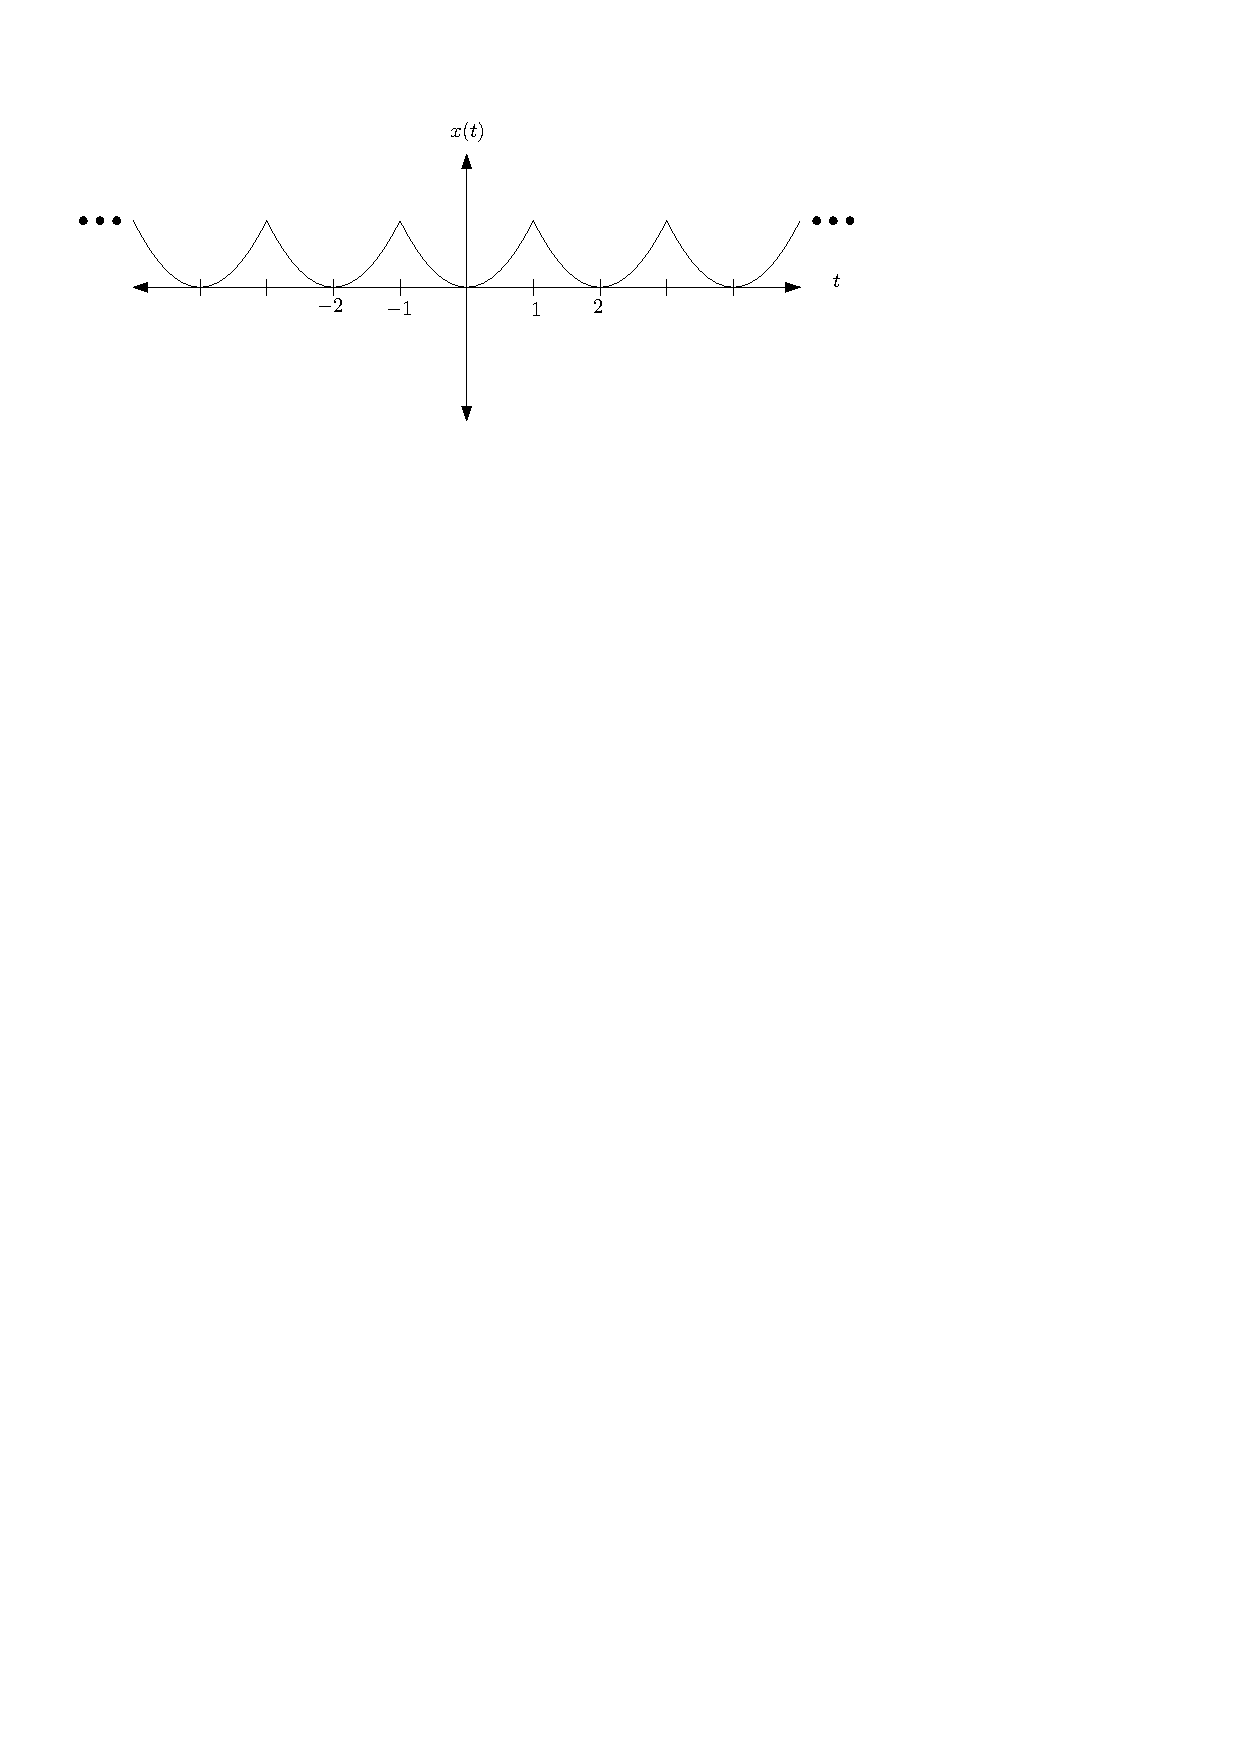
\includegraphics[scale=1]{graphics/ctfs-example1.pdf}
\end{center}
To find the Fourier Series approximation of $x(t)$,
\[
x(t) \approx \sum\limits_{k = -\infty}^{\infty} a_k \, e^{j k\omega_0 t}\; ,
\]
we need to find the coefficients
\[
a_k = \frac{1}{T_0} \int\limits_{0}^{T_0} x(t)e^{-jk\omega_0 t} \; dt
\]
Since the integration can be over any period, we can use the limits $[-1,1]$ and note that $T_0 = 2$ so that $\omega_0 = \pi$, giving the sequence of expressions
\begin{align*}
  a_k &= \frac{1}{2} \int\limits_{-1}^{1} t^2\,e^{-jk\pi t} \; dt\\
  &= \frac{1}{2} \left[ \int\limits_{-1}^{1} t^2\,\cos(-k\pi t) \; dt + j \int\limits_{-1}^{1} t^2\,\sin(-k\pi t) \; dt \right]\\
  &= \frac{1}{2} \left[ \int\limits_{-1}^{1} t^2\,\cos(k\pi t) \; dt + j \int\limits_{-1}^{1} - t^2\,\underbrace{\sin(k\pi t)}_{\text{always = 0}} \; dt \right]\\
  &= \frac{1}{2} \int\limits_{-1}^{1} t^2\,\cos(k\pi t) \; dt\; \mbox{ using an integration table }\\
  &= \frac{1}{2} \frac{4k\pi\overbrace{\cos(k\pi)}^{(-1)^k} + 2(k^2\pi^2-2)\overbrace{\sin(k\pi)}^{\text{always = 0}}}{k^3\pi^3}\\
 a_k &= \frac{2}{k^2\pi^2}\left(-1\right)^k
\end{align*}
This result is undefined for when $k=0$. In that case note the original integral is
\[
a_0 = \frac{1}{2} \int\limits_{-1}^{1} t^2 \; dt = \frac{1}{6}t^3 \Big|_{-1}^{1} = \frac{1}{3} 
\]
Thus the final approximation is
\[
x(t) \approx \sum\limits_{k = -\infty}^{\infty} \underbrace{\frac{2}{k^2\pi^2}\left(-1\right)^k}_{a_k} \, e^{j k\pi t} \;.
\]
We can plot the spectrum of this signal (using for example Matlab)
\begin{verbatim}
k = -10:10;
a = 2./(pi^2*k.^2);
a(11) = 1/3;

subplot(2,1,1);
stem(k, abs(a));
xlabel('k');
ylabel('|a(k)|');
title('Amplitude Spectrum');

subplot(2,1,2);
stem(k, angle(a));
xlabel('k');
ylabel('Angle a(k)');
title('Phase Spectrum');
\end{verbatim}
Giving the amplitude and phase spectrum plot
\begin{center}
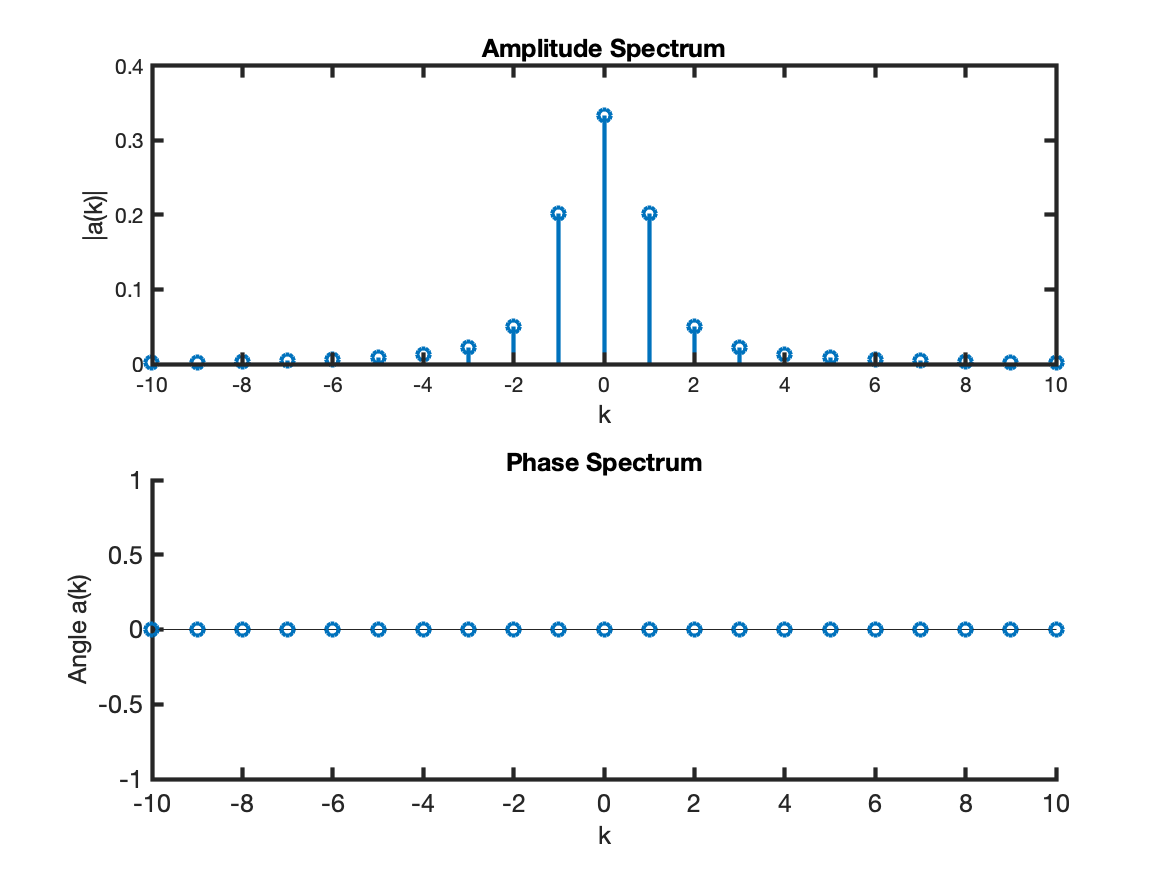
\includegraphics[scale=0.7]{graphics/ctfs_exampleplot.png}
\end{center}
$\blacksquare$
\end{example}

\subsection{Variations on the Synthesis and Analysis Equations}
There are two commonly used, equivalent, expressions for computing the CTFS coefficients. They can be derived using Euler's formula and related trig identities.

\begin{itemize}
\item Exponential Form. This is the form derived above
  \[
  x(t) = \sum\limits_{k = -\infty}^{\infty} a_k \, e^{j k\omega_0 t}
  \]
  where 
  \[
  a_k = \frac{1}{T_0} \int\limits_{T_0} x(t)e^{-jk\omega_0 t} \; dt
  \]
\item Trig Form
  \[
  x(t) = b_0 + \sum\limits_{k = 1}^{\infty} b_k \,\cos(k\omega_0 t) + c_k\,\sin(k\omega_0 t) 
  \]
  where
  \[
  b_0 = \frac{1}{T_0} \int\limits_{T_0} x(t) \; dt
  \]
  is the average value of the signal, and
  \[
  b_k = \frac{2}{T_0} \int\limits_{T_0} x(t)\cos(k\omega_0 t) \; dt
  \]
  \[
  c_k = \frac{2}{T_0} \int\limits_{T_0} x(t)\sin(k\omega_0 t) \; dt
  \]
\item Compact Trig Form
  \[
  x(t) = d_0 + \sum\limits_{k = 1}^{\infty} d_k \,\cos(k\omega_0 t + \theta_k) 
  \]
  where
  \[
  d_0 = \frac{1}{T_0} \int\limits_{T_0} x(t) \; dt
  \]
  is the average value of the signal, and
  \[
  d_k = \sqrt{b_k^2 + c_k^2} 
  \]
  \[
  \theta_k = \arctan\left( \frac{-c_k}{b_k} \right)
  \]
\end{itemize}

\subsection{Convergence of the CT Fourier Series}

As mentioned above the Fourier Series is strictly speaking an approximation
\[
x(t) \approx \sum\limits_{k = -\infty}^{\infty} a_k \, e^{j k\omega_0 t} \mbox{ where } a_k = \frac{1}{T_0} \int\limits_{T_0} x(t)e^{-jk\omega_0 t} \; dt
\]
to determine when this approximation is an equivalence (and in what sense) we need to establish the existence and convergence of the integral and summation respectively.

The coefficients $a_k$ will exist when the integral converges, or equivalently when
\[
\int\limits_{T_0} \left|x(t)\right| \; dt < \infty
\]
i.e. the signal is absolutely integrable over any period. Note, such a signal is a power signal.

To determine when the summation converges, first consider the \emph{truncated} CT Fourier Series
\[
x_N(t) \approx \sum\limits_{k = -N}^{N} a_k \, e^{j k\omega_0 t}
\]
where the infinite sum has been truncated to the finite range $[-N,N]$. Define the error between the original signal $x(t)$ and the truncated approximation $x_N(t)$ at each time point as
\[
E(N,t) = x(t) - x_N(t)
\]
There are two relevant notions of convergence. If
\[
\lim_{N\rightarrow \infty} \int\limits_{T_0} \left| E(N,t] \right|\;dt = 0
\]
we say the CT Fourier Series converges \emph{exactly} to the signal. If
\[
\lim_{N\rightarrow \infty} \int\limits_{T_0} \left| E(N,t) \right|^2\;dt = 0
\]
we say the CT Fourier Series converges in the \emph{mean-square} sense to the signal.

More formally the CTFS exists if the \emph{Dirichlet Conditions} hold for the signal:

\begin{itemize}
\item The signal has a finite number of discontinuities per period.
\item The signal has a finite number of maxima and minima per period.
\item The signal is bounded, i.e.
  \[
  \int_{T_0} |x(t)| \;dt < \infty
  \]
\end{itemize}

These conditions rule out pathological functions. For most practical signals of interest, the conditions hold.

\begin{example}
  Consider the \emph{impulse train} signal defined as
  \[
  x(t) = \sum\limits_{m = -\infty}^{\infty} \delta(t-mT_0)
  \]
  which we be important later when we discuss sampling CT signals. Do the Dirichlet conditions hold? Yes. It has one discontinuity, one maximum, and one minimum per period. It is also bounded since
  \[
  \int_{T_0} |\delta(t)| \;dt = 1 \mbox{ by definition.}
  \]
  The spectrum for the impulse train is given by
  \[
  a_k = \frac{1}{T_0} \int\limits_{T_0} x(t)e^{-jk\omega_0 t} \; dt =  \frac{1}{T_0} \int\limits_{-\frac{T_0}{2}}^{\frac{T_0}{2}} \delta(t)e^{-jk\omega_0 t} \; dt = \frac{1}{T_0}
  \]
  $\blacksquare$
\end{example}


\begin{example}
  Consider the signal $x(t) = \cos(\omega t)$. We can write this as the sum of two complex exponentials using Euler's formula
  \[
  x(t) = \frac{1}{2}e^{j\omega t} + \frac{1}{2}e^{-j\omega t} 
  \]
  Comparing this to the synthesis equation
  \[
  x(t) = \sum\limits_{k = -\infty}^{\infty} a_k \, e^{j k\omega_0 t} = \cdots + a_{-2} \, e^{j (-2)\omega_0 t} + a_{-1} \, e^{j (-1)\omega_0 t} + a_0 + a_{1} \, e^{j (1)\omega_0 t} + a_{2} \, e^{j (2)\omega_0 t} + \cdots
  \]
  we note that if $\omega_0 = \omega$ and 
  \[
  a_k = \left\{ \begin{array}{lc}
    \tfrac{1}{2} & k = -1\\[0.5em]
    \tfrac{1}{2} & k = 1\\[0.5em]
    0 & \text{else}
  \end{array}
  \right.
  \]
  then the two expressions are identical and the CT Fourier Series is an exact representation.\\
  $\blacksquare$
\end{example}

\begin{example}
  Consider the square wave signal of amplitude $A > 0$
  \[
  x(t) = \sum\limits_{m= -\infty}^{\infty} \left\{ \begin{array}{lc}
    -A & \tfrac{T_0}{2} < t-mT_0 < 0\\[0.5em]
    A & 0 < t - mT_0 < \tfrac{T_0}{2}
  \end{array}
  \right.
  \]
  shown below
  \begin{center}
  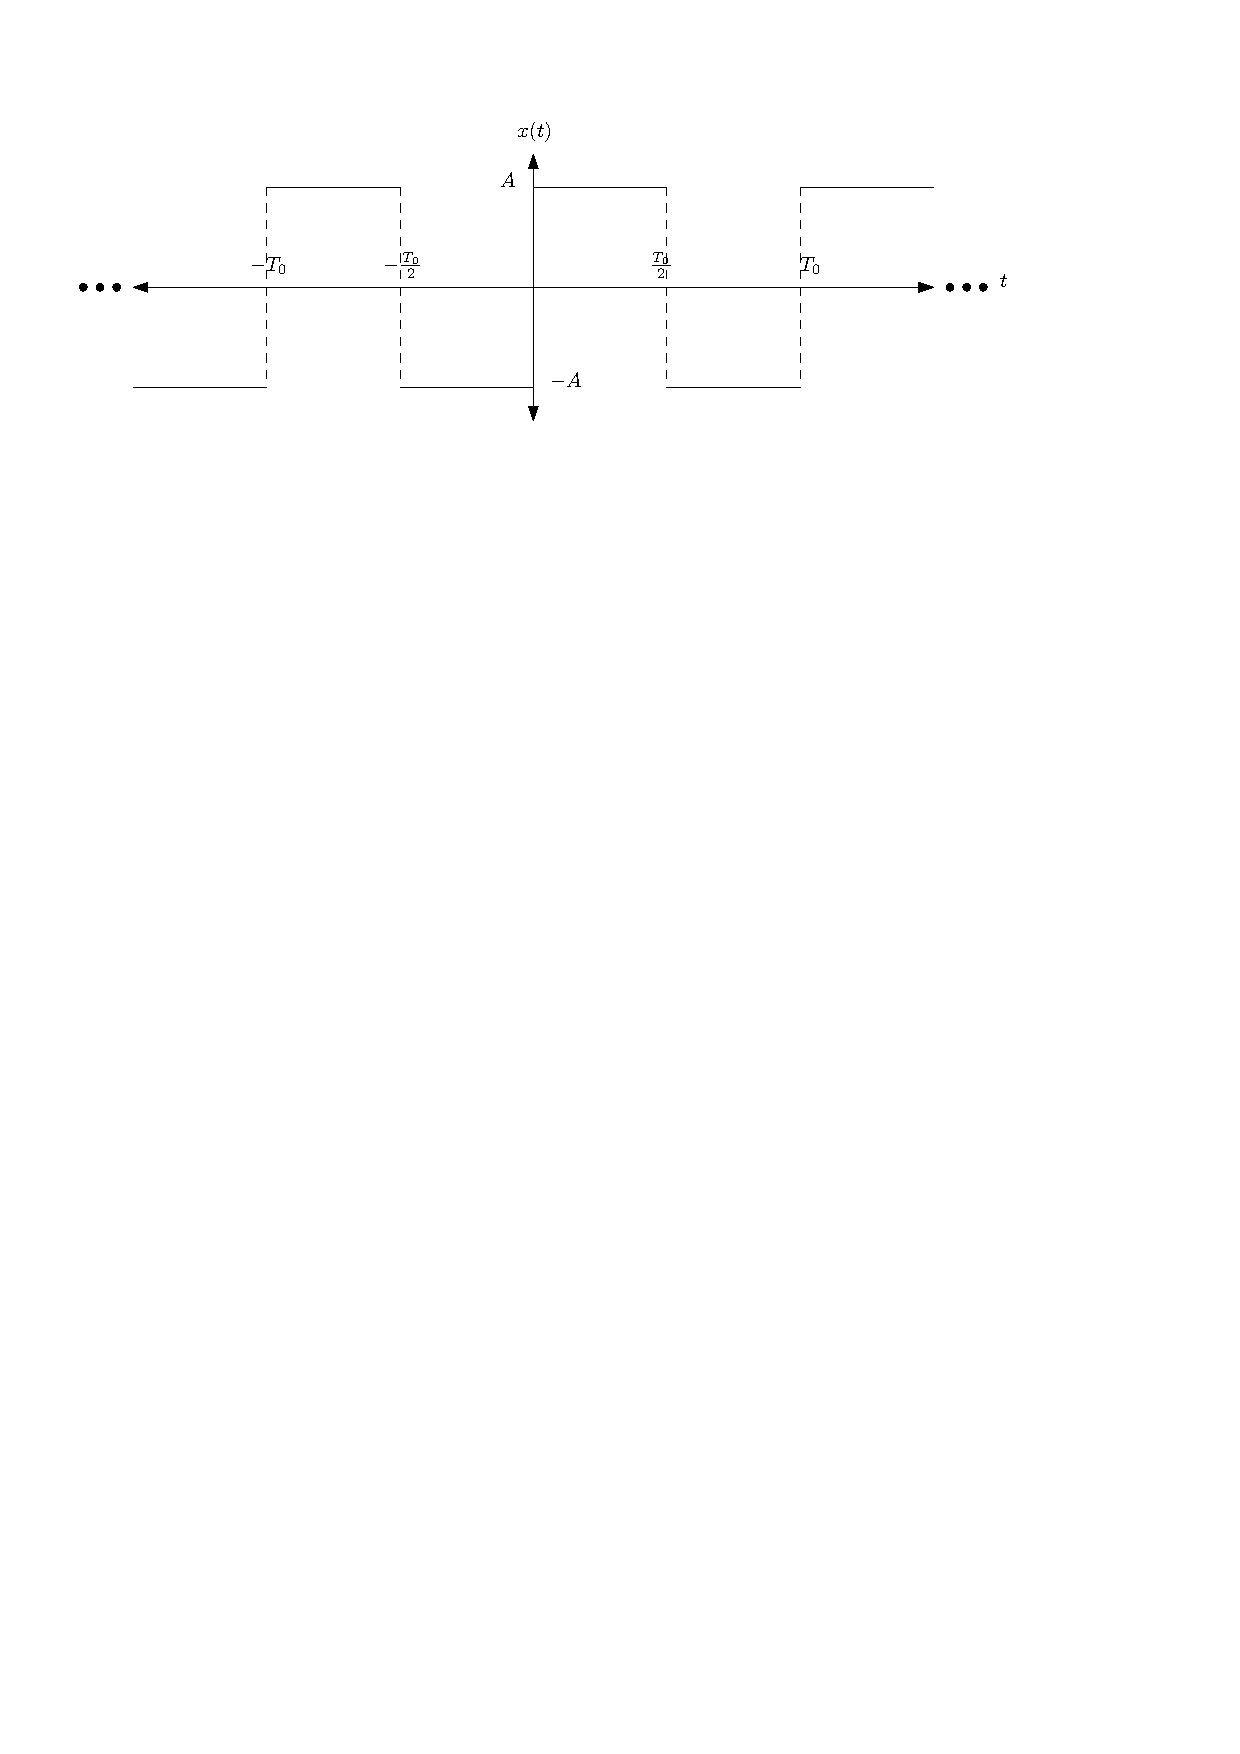
\includegraphics[scale=1]{graphics/squarewave.pdf}
  \end{center}
  The coefficients are given by
  \begin{align*}
    a_k &= \frac{1}{T_0} \int\limits_{T_0} x(t)e^{-jk\omega_0 t} \; dt\\
    &= \frac{1}{T_0} \left[ \int\limits_{0}^{\frac{T_0}{2}} Ae^{-jk\omega_0 t} \; dt + \int\limits_{\frac{T_0}{2}}^{T_0} -Ae^{-jk\omega_0 t} \; dt\right]\\
    &= \frac{1}{T_0} \left[ \frac{A}{-jk\omega_0}e^{-jk\omega_0 t} \Big|_{0}^{\frac{T_0}{2}} + \frac{-A}{-jk\omega_0}e^{-jk\omega_0 t} \Big|_{\frac{T_0}{2}}^{T_0}\right]\\
    &= \frac{1}{T_0} \frac{A}{jk\omega_0} \left[ -\left(e^{-jk\omega_0 \frac{T_0}{2}} - e^{0}\right) + \left(e^{-jk\omega_0 T_0} - e^{-jk\omega_0 \frac{T_0}{2}}\right)\right]
  \end{align*}
  Note that $\omega_0\frac{T_0}{2} = \frac{2\pi}{T_0}\frac{T_0}{2}= \pi$ and $\omega_0 T_0 = \frac{2\pi}{T_0}T_0 = 2\pi$ . Thus
  \begin{align*}
    a_k &= \frac{1}{T_0} \frac{A}{jk\frac{2\pi}{T_0}} \left[ -\left(e^{-jk\pi} - e^{0}\right) + \left(e^{-jk2\pi} - e^{-jk\pi}\right)\right]\\
    &= \frac{A}{jk\pi}\left( 1-e^{-jk\pi}\right) \\
    &= \left\{ \begin{array}{lc}
      0 & k \mbox{ even}\\
      \frac{2A}{jk\pi} & k \mbox{ odd}
    \end{array}
\right.
  \end{align*}
  The amplitude spectrum is given by
  \[
  |a_k| = \left\{ \begin{array}{lc}
    0 & k \mbox{ even}\\
    \left|\frac{2A}{k\pi}\right| & k \mbox{ odd}\end{array}\right.
  \]

  The phase spectrum is given by
  \[
  \angle a_k = \left\{ \begin{array}{lc}
    \pi & k < 0 \mbox{ and even}\\
    -\pi & k > 0 \mbox{ and even}\\
    \frac{\pi}{2} & k < 0 \mbox{ and odd}\\
    -\frac{\pi}{2} & k > 0 \mbox{ and odd}\end{array}\right.
  \]
  This is plotted below for $A = 1$.
  \begin{center}
    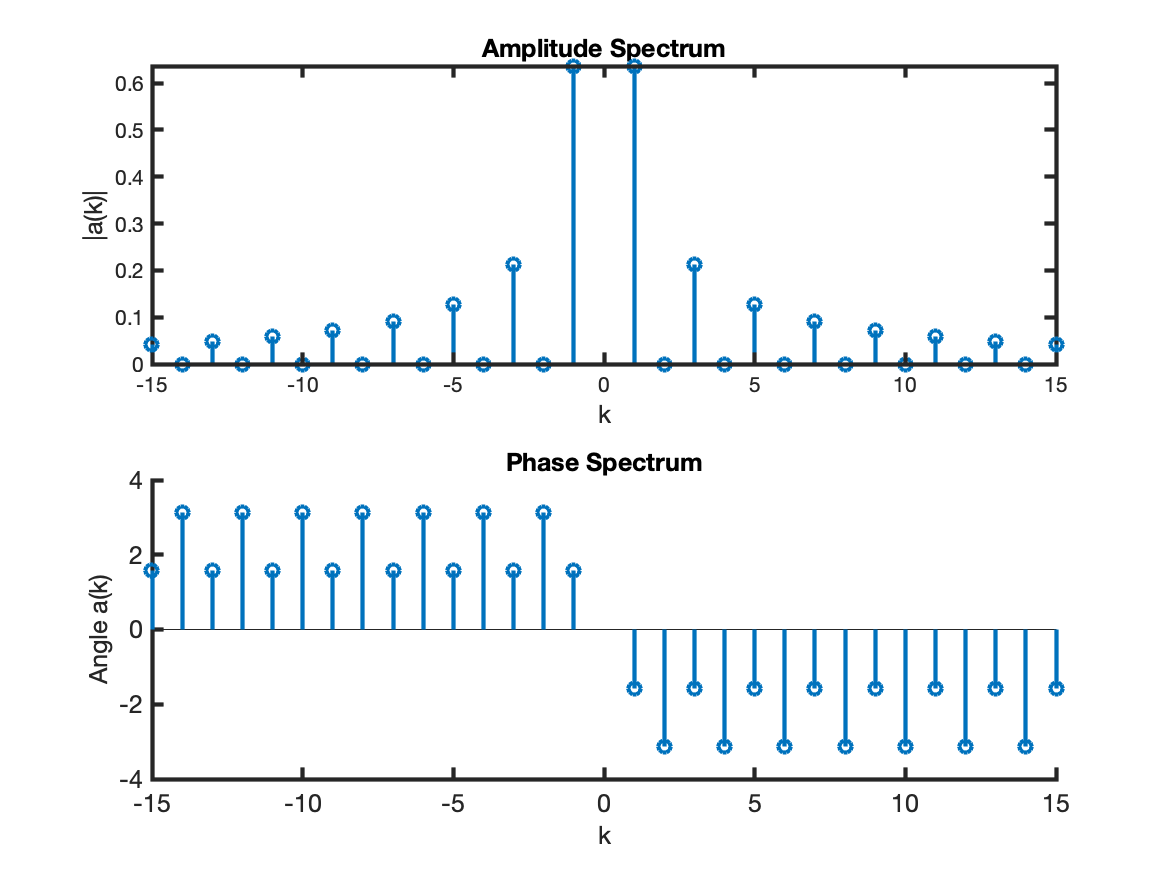
\includegraphics[scale=0.7]{graphics/ctfs_exampleplot2.png}
  \end{center}
  We can plot the truncated approximation for increasing number of terms N, the squared error, and the total error.
  \begin{center}
    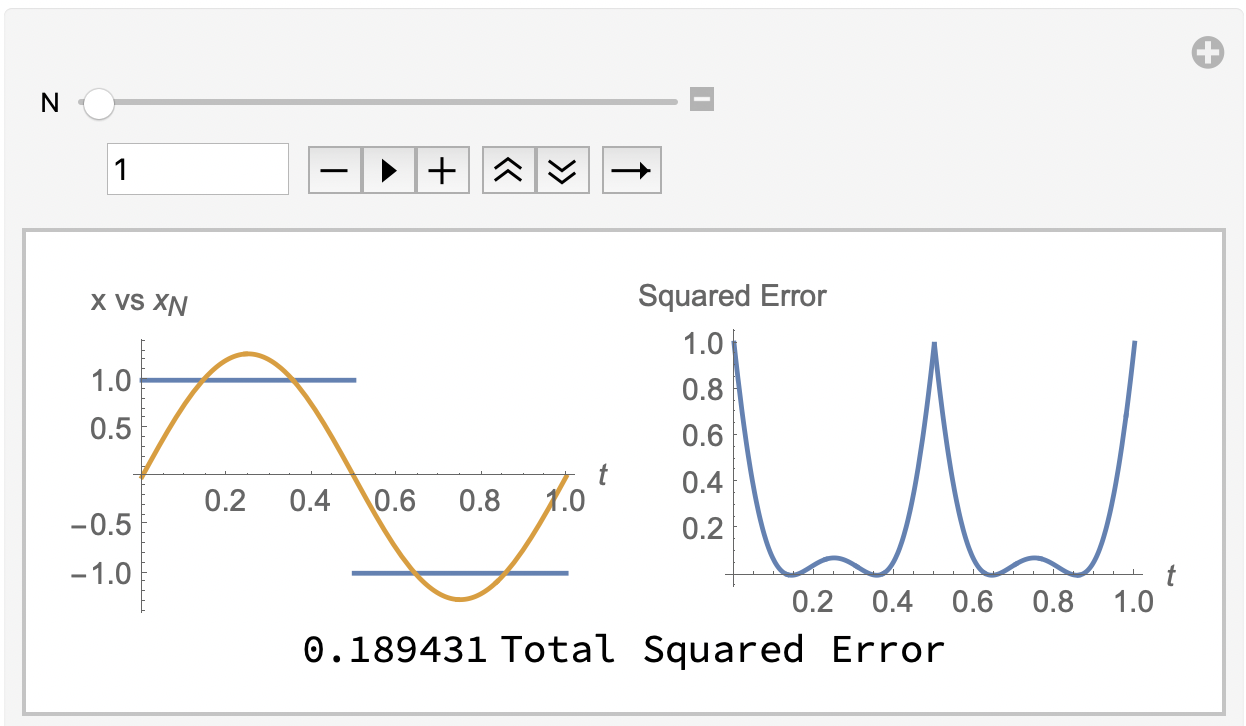
\includegraphics[scale=0.5]{graphics/squarewaveapprox1.png}
  \end{center}
  \begin{center}
    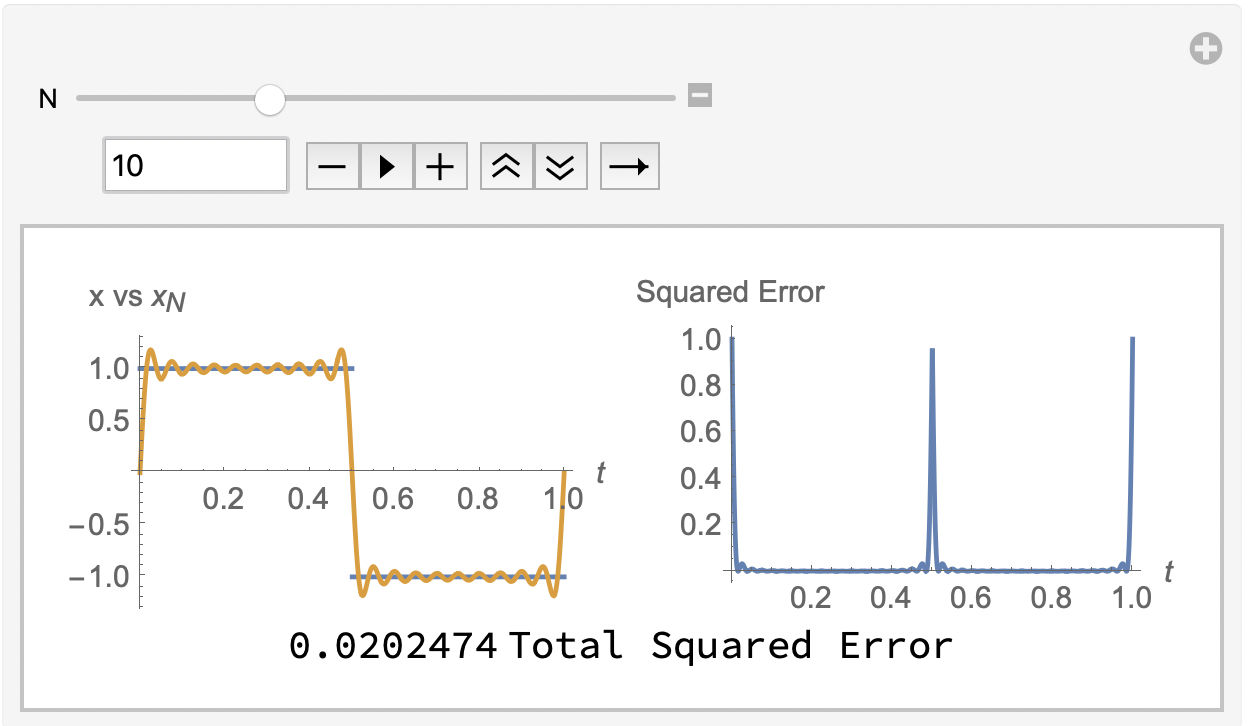
\includegraphics[scale=0.5]{graphics/squarewaveapprox2.png}
  \end{center}
  \begin{center}
    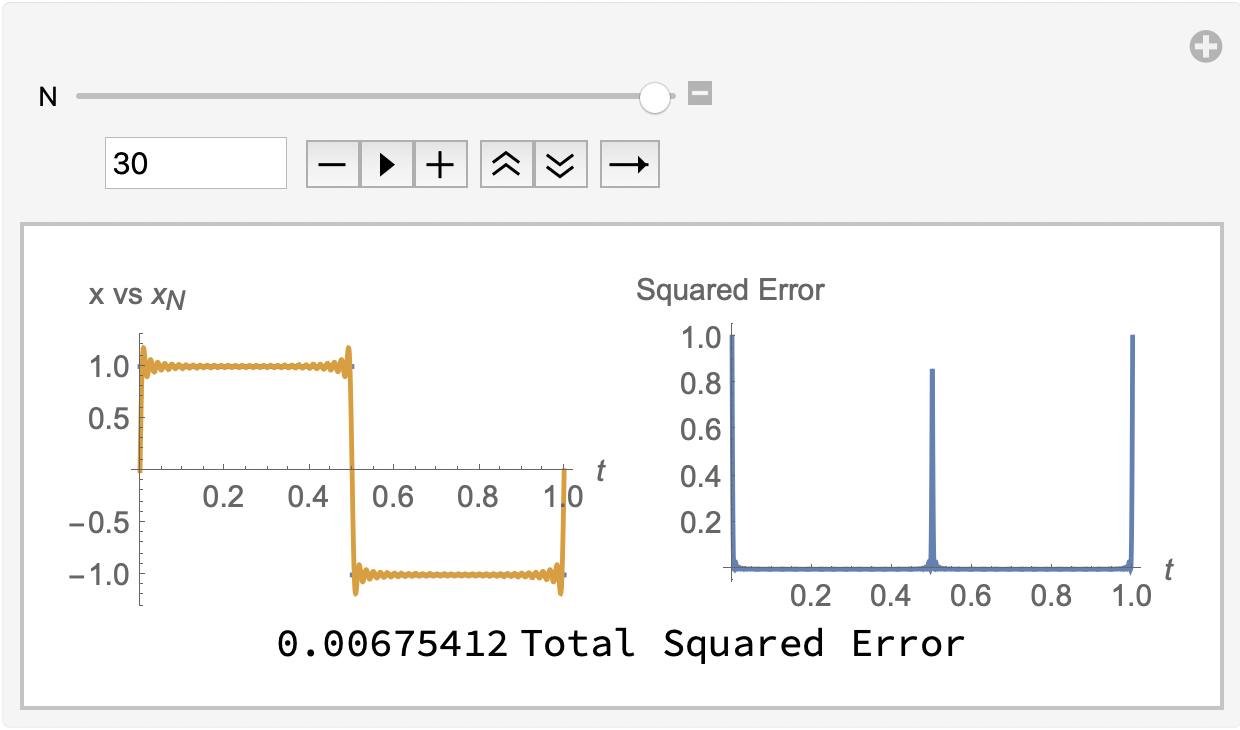
\includegraphics[scale=0.5]{graphics/squarewaveapprox3.png}
  \end{center}
  Note as $N$ increases the approximation gets closer to the square wave, except at the discontinuities. This is called \emph{Gibbs Ringing}. As $N \rightarrow \infty$ the mean-square error goes to zero, so the CTFS approximation to the square wave converges in the mean-square sense.
  $\blacksquare$
\end{example}


\subsection{Properties of the CT Fourier Series}

Let $a_k$ and $b_k$ be the CTFS coefficients for the periodic signals $x(t)$ and $y(t)$ respectively.

\begin{itemize}
\item Linearity. The coefficients of the signal
  \[
  z(t) = Ax(t) + By(t) \mbox{ for constants } A,B 
  \]
  are $Aa_k + Bb_k$
\item Time Shifting. The coefficients of
  \[
  z(t) = x(t-t_0) \mbox{ are } e^{-jk\omega_0 t_0}a_k
  \]
  that is it adds a phase shift.
\item Time reversal. The coefficients of
  \[
  z(t) = x(-t) \mbox{ are } a_{-k}
  \]
  that is the sequence reverses.
\item Time Scaling. Let $T_0$ and $\omega_0$ be the fundamental period and frequency of a periodic $x(t)$. The signal 
  \[
  z(t) = x(\alpha t) \mbox{ for } \alpha > 0
  \]
  is periodic with period $\frac{T_0}{\alpha}$ and fundamental frequency $\alpha\omega_0$.
  The coefficients of $z(t)$ are the same as $x(t)$.
\item Multiplication. The coefficients of
  \[
  z(t) = x(t) \cdot y(t) \mbox{ are } \sum\limits_{m = -\infty}^{\infty} a_m\cdot b_{k-m}
  \]
  the discrete convolution of the individual signals' coefficients.
\item Conjugate Symmetry. The coefficients of
  \[
  z(t) = x^*(t) = \Re{x(t)} - j\Im{x(t)} \mbox{ are } a_{-k}^*
  \]
  A consequence of this property is that real, even signals have real, even $a_k$; and real, odd signals have purely imaginary, odd $a_k$ (check the examples above).
\item Parseval's Relation. The power of the signal with Fourier series coefficients
  \[
  \frac{1}{T_0} \int_{T_0} |x(t)|^2\;dt = \sum\limits_{k = -\infty}^{\infty} |a_k|^2
  \]
\end{itemize}


%\subsection{Applications of the CT Fourier Series}

%TODO example of recitifier
